\begin{figure}[h]
    \centering
    \begin{subfigure}[b]{0.9\textwidth}
        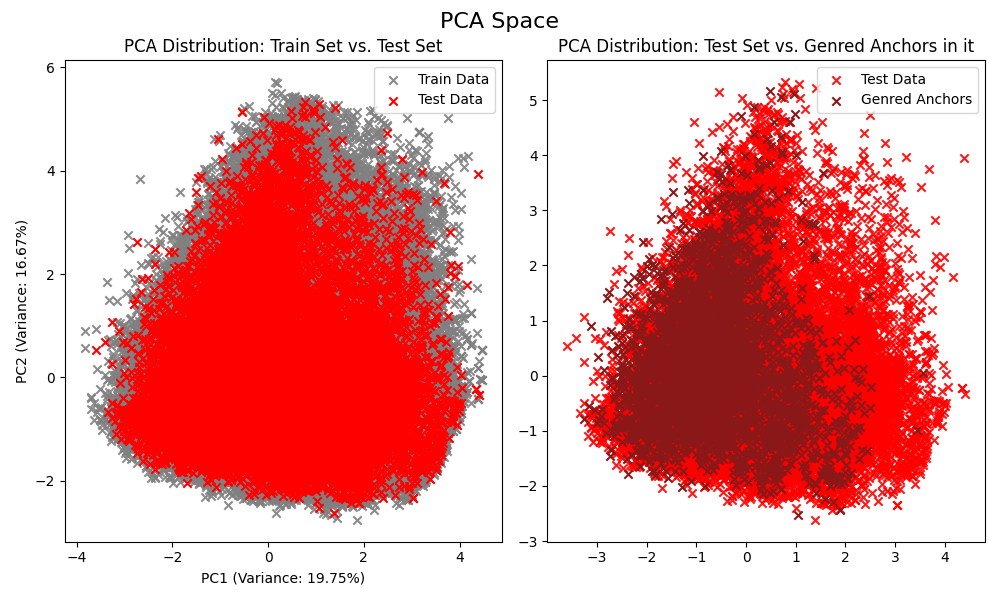
\includegraphics[width=\textwidth]{Images/pca/pca_xg_ca_anchors.png}
        \caption{Model: XGBoost, XAI method: Anchors}
        \label{fig:pca_xg_ca_anchors}
    \end{subfigure}
    \hfill
    \begin{subfigure}[b]{0.9\textwidth}
        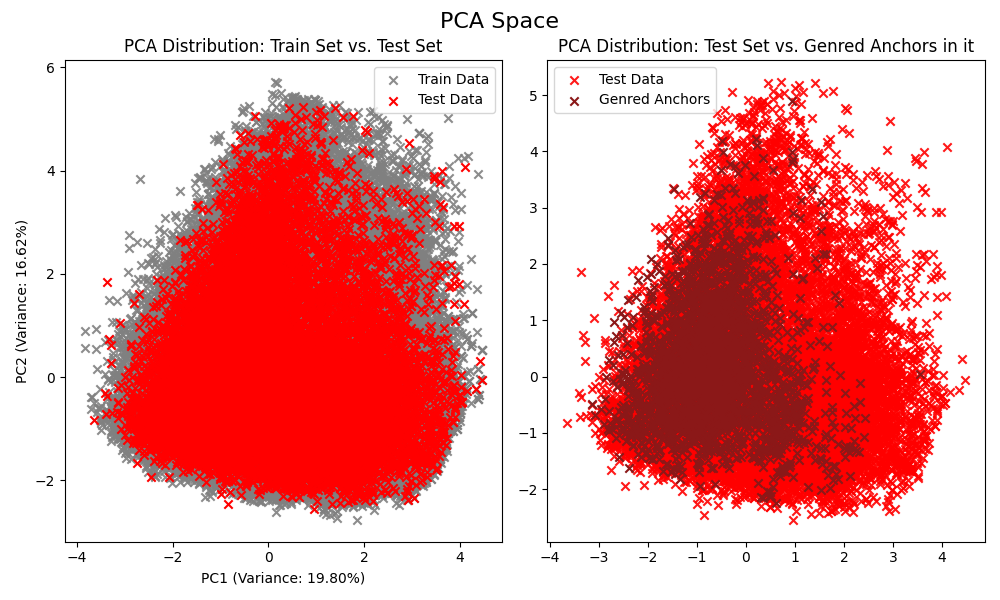
\includegraphics[width=\textwidth]{Images/pca/pca_skrub_ca_anchors.png}
        \caption{Model: HistGradientBoosting, XAI method: Anchors}
        \label{fig:pca_skrub_ca_anchors}
    \end{subfigure}
    \caption{PCA of the test dataset in the California state (Part 1)}
 \end{figure}

\begin{figure}[h]
    \ContinuedFloat
    \begin{subfigure}[b]{0.9\textwidth}
        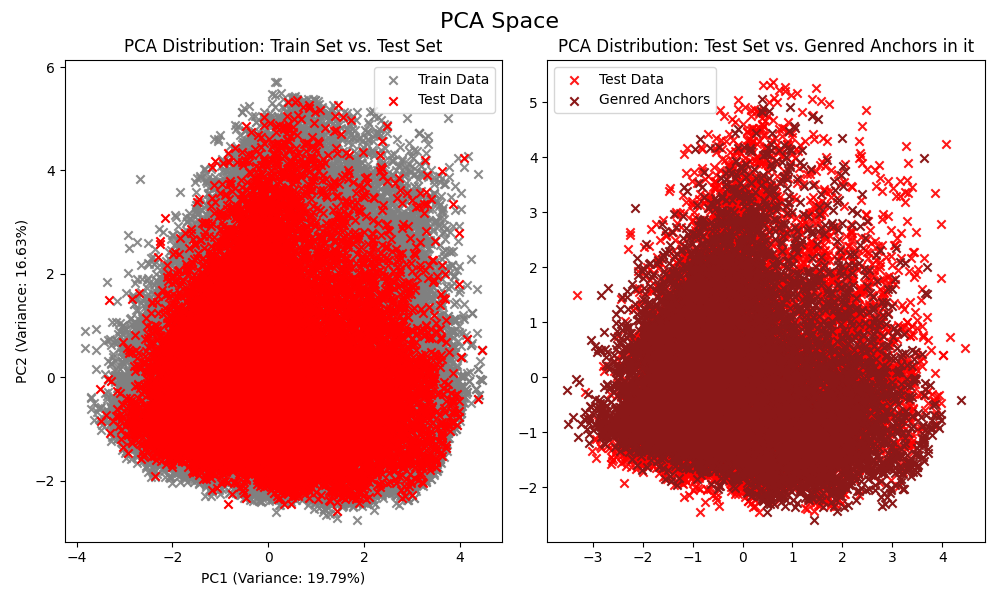
\includegraphics[width=\textwidth]{Images/pca/pca_xg_ca_shap.png}
        \caption{Model: XGBoost, XAI method: SHAP}
        \label{fig:pca_xg_ca_shap}
    \end{subfigure}
    \hfill
    \begin{subfigure}[b]{0.9\textwidth}
        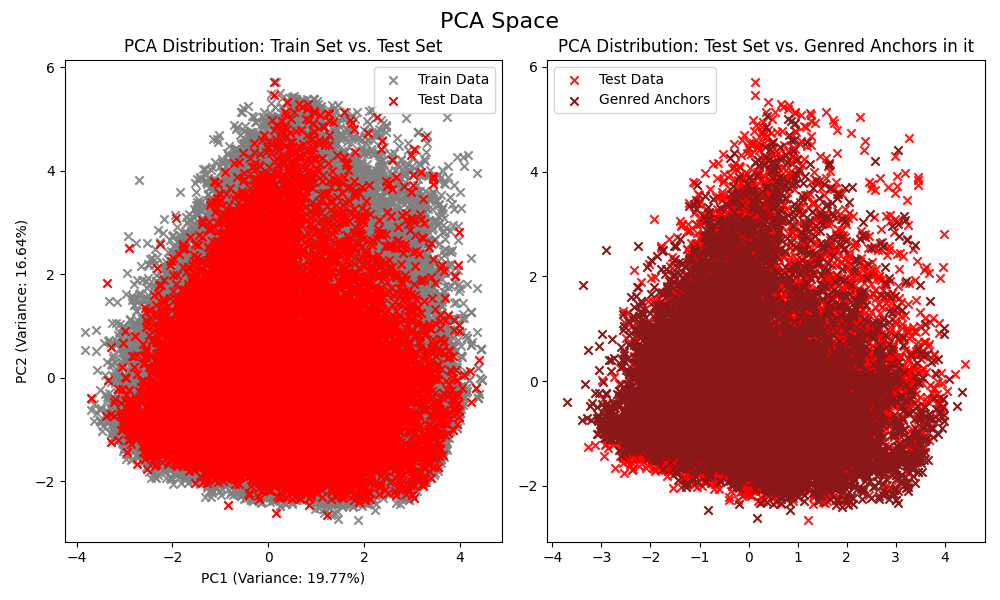
\includegraphics[width=\textwidth]{Images/pca/pca_skrub_ca_shap.png}
        \caption{Model: HistGradientBoosting, XAI method: SHAP}
        \label{fig:pca_skrub_ca_shap}
    \end{subfigure}
    \caption{PCA of the test dataset in the California state (Part 2)}
    \label{fig:pca_ca}
\end{figure}
    


\begin{figure}[h]
    \centering
    \begin{subfigure}[b]{0.9\textwidth}
        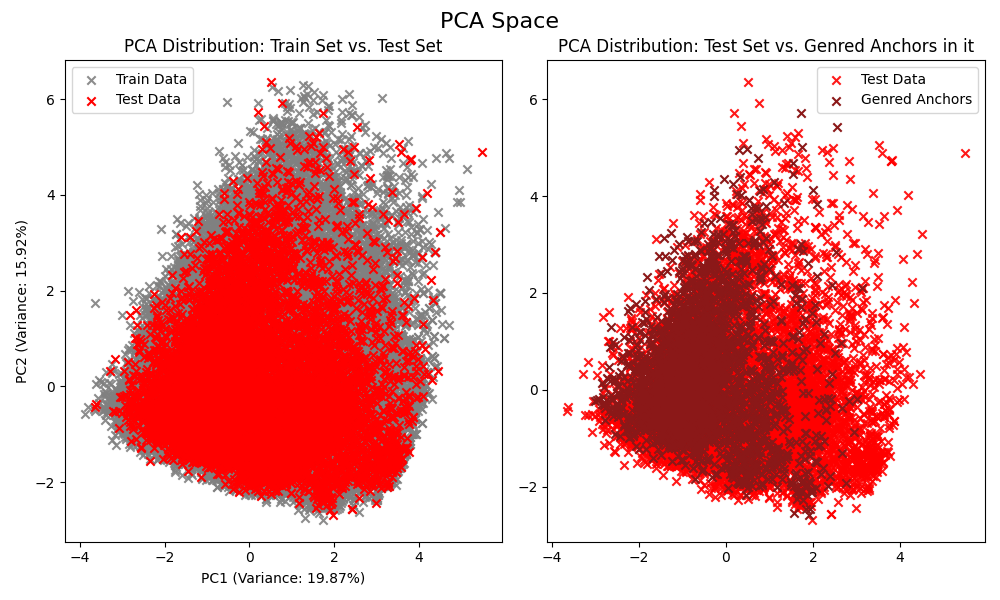
\includegraphics[width=\textwidth]{Images/pca/pca_xg_ny_anchors.png}
        \caption{Model: XGBoost, XAI method: Anchors}
        \label{fig:pca_xg_ny_anchors}
    \end{subfigure}
    \hfill
    \begin{subfigure}[b]{0.9\textwidth}
        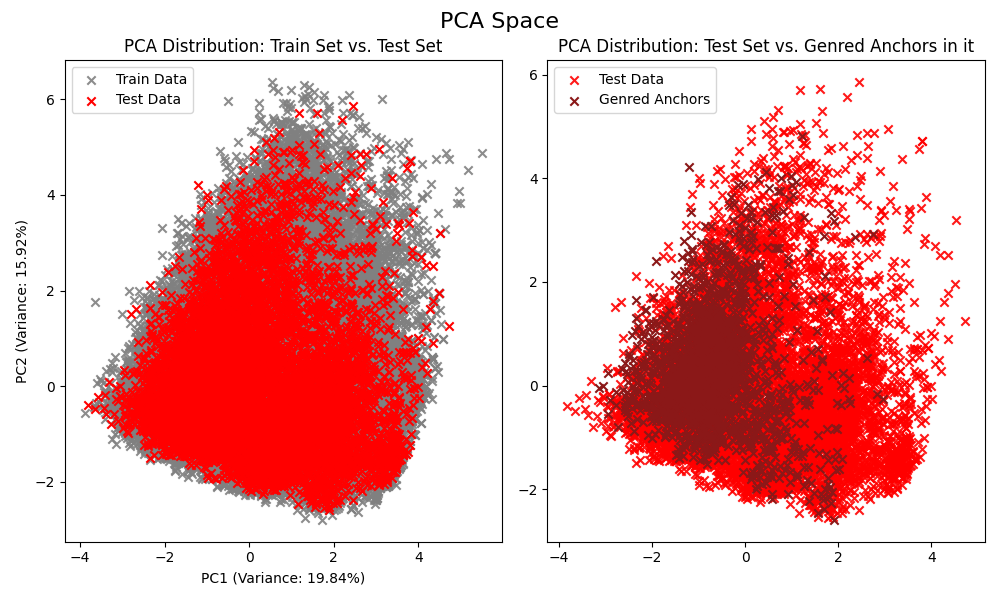
\includegraphics[width=\textwidth]{Images/pca/pca_skrub_ny_anchors.png}
        \caption{Model: HistGradientBoosting, XAI method: Anchors}
        \label{fig:pca_skrub_ny_anchors}
    \end{subfigure}
\caption{PCA of the test dataset in the New York state (Part 1)}
 \end{figure}

\begin{figure}[h]
    \ContinuedFloat
    \begin{subfigure}[b]{0.9\textwidth}
        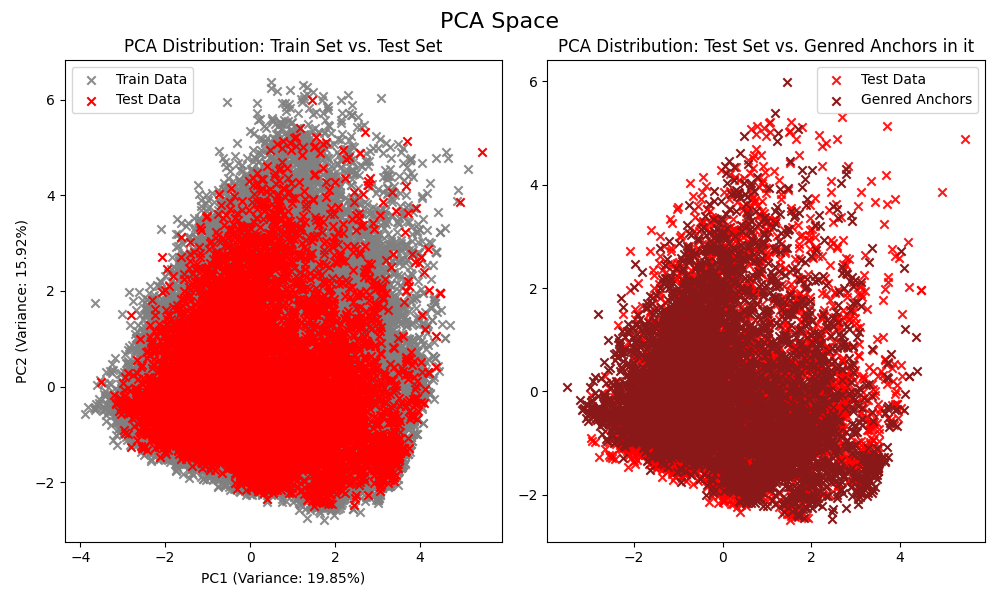
\includegraphics[width=\textwidth]{Images/pca/pca_xg_ny_shap.png}
        \caption{Model: XGBoost, XAI method: SHAP}
        \label{fig:pca_xg_ny_shap}
    \end{subfigure}
    \hfill
    \begin{subfigure}[b]{0.9\textwidth}
        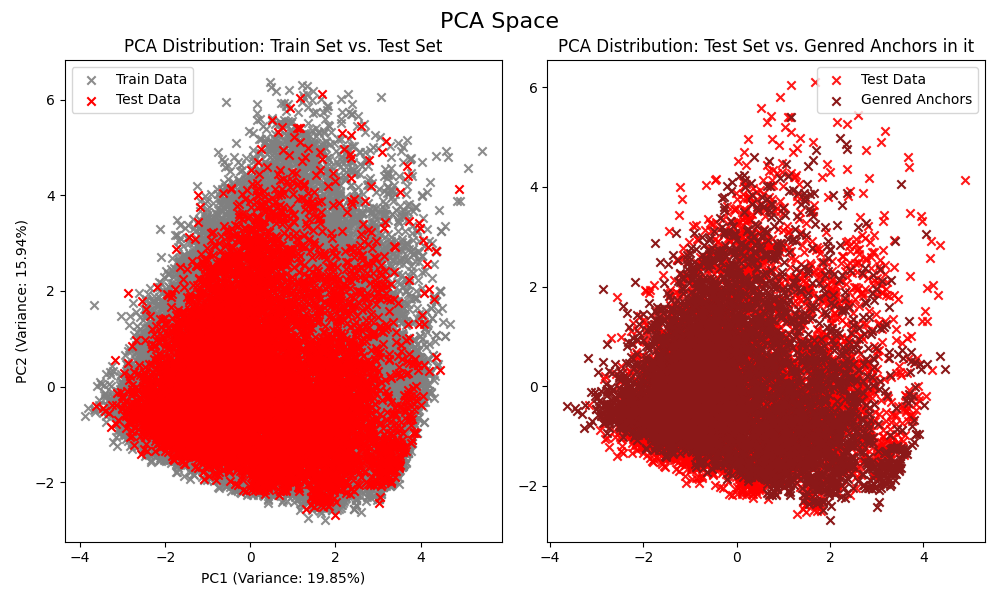
\includegraphics[width=\textwidth]{Images/pca/pca_skrub_ny_shap.png}
        \caption{Model: HistGradientBoosting, XAI method: SHAP}
        \label{fig:pca_skrub_ny_shap}
    \end{subfigure}
    \caption{PCA of the test dataset in the New York state (Part 2)}
    \label{fig:pca_ny}
\end{figure}